\chapter{Protótipo AFD e Plano de Testes}

Esse capítulo apresenta a arquitetura e a implementação de um protótipo para o AFD (Assentamento Funcional Digital) que objetiva servir para a investigação proposta nesse trabalho e descrita na introdução. Primeiro serão descritas as principais características do projeto como tecnologias utilizadas e arquitetura proposta e,  para finalizar o capítulo, serão descritos os planos de testes que foram desenvolvidos para os testes de performance.

\section{O Protótipo}

Para a execução dos testes de performance foi desenvolvido uma aplicação orientada a serviços ~\cite{erl:2007} com as principais capacidades necessárias para manter os dados do AFD. O objetivo central da aplicação é manter os documentos da pasta funcional dos servidores. Como a aplicação deve armazenar aquivos digitalizados, escolhemos gravar o arquivo no sistema operacional e armazenar o caminho para ele na base de dados. O objetivo ao se escolher realizar os testes de performance em uma arquitetura orientada a serviços foi o de flexibilizar ao máximo as implementações em diversos bancos de dados. Na tabela \ref{tab:funcionalidades} a descrição das funcionalidades implementadas.

\renewcommand{\arraystretch}{3}

\begin{table}
	\caption{Descrição das Funcionalidades}
	\begin{center}
	\begin{tabularx}{\textwidth}{ | c | X | }
		\hline
			\textbf{Funcionalidade} & \multicolumn{1}{c|}{\textbf{Descrição}} \\
		\hline
			Insere Orgão & \noindent\parbox[c]{\hsize}{Permite inserir as unidades pagadoras ou orgãos que terão os dados dos empregados mantidos no sistema.} \\
		\hline
			Insere Empregado & \noindent\parbox[c]{\hsize}{Permite inserir os empregados de cada orgão.} \\
		\hline
			Insere Dependente & \noindent\parbox[c]{\hsize}{Permite inserir os dependentes de cada empregado.}\\
		\hline
			Insere Documento Dependente & \noindent\parbox[c]{\hsize}{Permite inserir os documentos dos dependentes que farão parte da pasta funcional do empregado.} \\
		\hline
			Insere Documento Empregado & \noindent\parbox[c]{\hsize}{Permite inserir os documentos que farão parte da pasta funcional do empregado.} \\
		\hline
			Lista Orgãos & \noindent\parbox[c]{\hsize}{Lista os dados dos órgãos cadastrados no sistema.} \\
		\hline
			Lista Empregados & \noindent\parbox[c]{\hsize}{Lista os dados dos empregados cadastrados no sistema.} \\
		\hline
			Lista Dependentes & \noindent\parbox[c]{\hsize}{Lista os dados dos dependentes dos empregados.} \\
		\hline
			Lista Documentos Empregados & \noindent\parbox[c]{\hsize}{Retorna os documentos da pasta funcional do empregado.} \\
		\hline
			Lista Documentos Dependentes & \noindent\parbox[c]{\hsize}{Retorna os documentos dos dependentes dos empregados.} \\
		\hline
			Relatório de Empregados Ativos & \noindent\parbox[c]{\hsize}{Calcula e exibe a quantidade de empregados ativos por orgão.} \\
		\hline
			Lista Vínculos & \noindent\parbox[c]{\hsize}{Lista os valores possíveis para os tipos de vínculos entre empregados e dependentes.} \\
		\hline
			Lista Tipo Documentos & \noindent\parbox[c]{\hsize}{Lista os valores possíveis para os tipos de documentos.} \\
		\hline
			Remove Dependente & \noindent\parbox[c]{\hsize}{Exclui o depente e seus arquivos.} \\
		\hline
			Desliga Empregado & \noindent\parbox[c]{\hsize}{Atualiza o status do empregado incluindo a data de desligamento.} \\
		\hline
	\end {tabularx}
	\end{center}
	%\caption{Fonte: http://docs.mongodb.org}
	\label{tab:funcionalidades}
\end{table}

\section{A Arquitetura do Projeto}

Para cumprirmos o nosso objetivo, que é testar a aplicação com um banco de dados relacional (PostgreSQL) e um banco de dados NoSQL orientado a documentos (MongoDB), montamos uma arquitetura simples, mas que nos permite trocar as implementações da camada de persistência sem maiores esforços. Para a execução dos testes utilizamos o JMeter. A aplicação foi desenvolvida em Python com o apoio do framework web2py na implementação do \textit{web service}. A linguagem de programação Python foi escolhida pela facilidade de encontrar drivers de diversos bancos de dados relacionais e não relacionais, além de ser uma linguagem orientada a objetos e de ampla utilização. O framework web2py foi adicionado ao projeto pelo motivo de suportar a implementação de \textit{web services} de modo rápido e fácil, além da geração automática do WSDL (arquivo que contém a descrição das operações do Web service). A diagramação da arquitetura pode ser vista na figura \ref{fig:arquitetura}

	\begin{figure}[!htbp]
		\begin{center}
			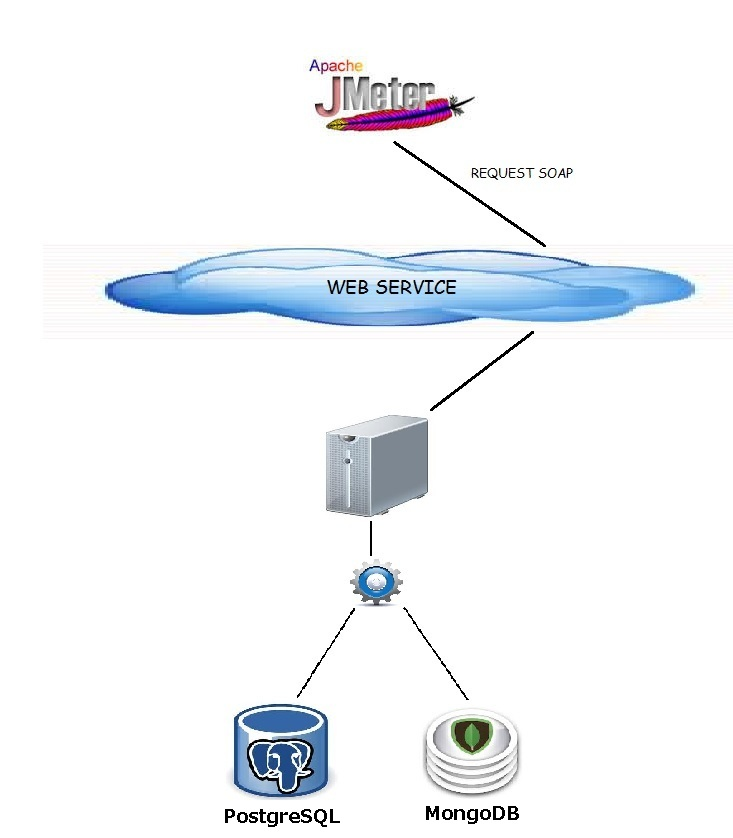
\includegraphics[width=0.5\textwidth]{arquitetura}
		\end{center}
		\caption{Arquitetura de Testes. JMeter faz requisições SOAP ao \textit{Web service} que pode estar configurado para persistir os dados no PostgreSQL ou no MongoDB.}
		\label{fig:arquitetura}
	\end{figure}

\subsection{web2py}

Web2py é um \textit{framework} para desenvolvimento ágil de aplicações web, software livre e gratuito. Ele é escrito e programável em Python. web2py foi inspirado pelo Ruby on Rails e Django. Tem seu foco no desenvolvimento ágil e segue o MVC (\textit{Model View Controller}). Toda aplicação web2py é composta por \textit{Models} (arquivos que contêm a descrição dos dados), \textit{Views} (arquivos que contêm a descrição dos dados que serão apresentados), \textit{Controlers} (arquivos que contêm a lógica e \textit{workflow} do negócio), \textit{Cron Jobs} (tarefas que precisam ser executadas regularmente) e \textit{Static Files} (imagens, \textit{scripts}, folhas de estilos, etc.) ~\cite{siteweb2py}.

Quando se trata de Web services, web2py oferece suporte para diversos protocolos, incluindo XML, JSON, RSS,CSV,XMLRPC,JSONRPC,AMFRPC, e SOAP.  O web2py inclui um cliente e servidor SOAP (pysimplesoap) criado por Mariano Reingart. Uma facilidade encontrada é a geração automática do WSDL e da página com a descrição das capacidades ~\cite{siteweb2py}.

\section{Os Planos de Teste}

Foi desenvolvido um plano de testes no JMeter para a maioria das funcionalidade da nossa aplicação. Os testes serão individualmente discutidos na seção de resultados do próximo capítulo. O testador utilizado no nosso projeto foi o de Requisição SOAP/XML - RPC. É nele que configuramos as requisições que serão feitas ao Web service da aplicação. Além de configurar uma requisição para cada plano de teste, temos como parametrizar outras configurações como a quantidade de usuários virtuais e o intervalo entre a iniciação de cada usuário. Na tabela \ref{tab:configplanoteste} temos as principais configurações dos nossos planos de teste. É importante realçar que todas as capacidades da nossa aplicação foram desenvolvidas para validarem os dados da mesma forma, ou seja, as regras de negócio verificadas, tanto usando o MongoDB quanto o PostgreSQL, são as mesmas. O passo a passo da execução dos planos de testes se dividem em dois tipos: Inserção/Exclusão/Atualização e Consulta.

\begin{table}
	\caption{Principais configurações dos Planos de Teste}
	\begin{center}
	\begin{tabularx}{\textwidth}{ | c | X | }
	\hline
		\textbf{Parâmetro} & \multicolumn{1}{c|}{\textbf{Descrição}} \\
	\hline
		Quantidade de usuários virtuais (threads) & Quanto maior o número de usuários virtuais, maior será o número de requisições simultâneas que a nossa aplicação terá que responder.\\
	\hline 
		Tempo de inicialização dos usuários virtuais & Indica o tempo total para a inicialização de todos os usuários virtuais. Para encontrarmos o tempo entre a inicialização de cada usuário devemos dividir pelo total de usuários virtuais.\\
	\hline
		O local dos arquivos CSV & Esses arquivos devem ser gerados antes do início dos testes com o apóio de um script.\\
	\hline
		Intervalo de medição dos gráficos & É o intervalo de tempo em que o JMeter faz as medidas para plotar cada gráfico.\\
	\hline
	\end {tabularx}
	\end{center}
	\label{tab:configplanoteste}
\end{table}

\subsection{Planos de Teste de Inserção/Exclusão/Atualização}

Os planos de Testes de Inserção executam os seguintes passos:

\begin{enumerate}
\item Configuração de Dados CSV - É indicado onde está o arquivo csv de onde as threads lerão os valores a serem enviados na requisição soap;
\item Requisição SOAP/XML-RPC - É configurada a URL do Web service e a requisição que será realizada. Cada requisição será montada com os dados lidos do arquivo csv. Cada thread lê uma linha diferente do arquivo.
\item Gráfico de Tempo de Resposta -  Elemento responsável por gerar um gráfico a partir dos dados da requisição feita. O gráfico exibe a  evolução do tempo de resposta das requisições feitas.
\item Gráfico de Resultados - Elemento responsável por exibir a evolução dos tempos das requisições, a média dos tempos das requisições, a derivação do tempo das requisições e a vazão.
\end{enumerate}

As funcionalidades que seguem esses passos são: insere órgão, insere empregado, insere dependente, insere documento dependente, insere documento empregado, desliga empregado e remove dependente.

Os testes que manipulam os arquivos da pasta funcional, devido à limitação da arquitetura disponível, e o teste de inserção de órgãos, devido a baixa massa de dados, só foram realizados para 10 e 100 usuários simultâneos. O restante foi executado para 10, 100 e 500 usuários simultâneos.

\subsection{Planos de Teste de Consulta}

Os planos de Testes de Consulta executam os seguintes passos:

\begin{enumerate}
\item Requisição SOAP/XML-RPC - É configurada a URL do Web service e a requisição que será realizada. Cada requisição será montada com os dados lidos do arquivo csv. Cada thread lê uma linha diferente do arquivo.
\item Gráfico de Tempo de Resposta -  Elemento responsável por gerar um gráfico a partir dos dados da requisição feita. O gráfico exibe a  evolução do tempo de resposta das requisições feitas.
\item Gráfico de Resultados - Elemento responsável por exibir a evolução dos tempos das requisições, a média dos tempos das requisições, a derivação do tempo das requisições e a vazão.
\end{enumerate}

As funcionalidades que seguem esses passos são: lista órgãos, lista empregados, lista dependentes, lista documentos dos empregados, lista documentos dos dependentes e relatório de empregados ativos.

Cada plano de teste de consulta foi executado durante um minuto. Os testes que manipulam os arquivos da pasta funcional, devido à limitação da arquitetura disponível, só foram realizados para 10 e 100 usuários simultâneos. O restante foi executado para 10,100 e 500 usuários simultâneos.